%% Intro

% Purpose
In this section we put either one or two middlewares between the \textit{memtier} clients and the \textit{memcached} servers. The purpose of this is to study the performance effects of our middleware. \\
% Experimental setup
The experimental setup is as follows: We let each experiment run for 80s and each experiment is repeated 3 times. The first and last 10 seconds of an experiment are considered to be unstable and are thus ignored. The standard deviation of a specific metric is computed over those repetitions and shown as error bars in the plots. From the outputs of the middleware we compute average queue length, a detailed breakdown of the response time and throughput of the middleware. In addition, the throughput and overall response time is computed from the outputs of the \textit{memtier} instances. Different kinds of resource usage statistics are computed with \textit{dstat}.

\subsection{One Middleware} \label{sec:baselineWithMWOne}
% setup description
In this setup we connect three load generator machines to a single middleware and use one memcached server. The overview of the experiment parameters is given in the following table:
\begin{center}
	\scriptsize{
		\begin{tabular}{|l|c|}
			\hline Number of servers                & 1                        \\ 
			\hline Number of client machines        & 3                        \\ 
			\hline Instances of memtier per machine & 1                        \\ 
			\hline Threads per memtier instance     & 2                        \\
			\hline Virtual clients per thread       & \{1,4,8,16,24,32\}  \\ 
			\hline Workload                         & Write-only and Read-only \\
			\hline Number of middlewares            & 1                        \\
			\hline Worker threads per middleware    & \{8,16,32,64\}             \\
			\hline Repetitions                      & 3                         \\ 
			\hline 
		\end{tabular}
	} 
\end{center}

$\bullet$ \textbf{Read-only load:} 
% plots
The throughput and response time as a function of virtual clients for read-only workloads is shown in Figure \ref{one_mw_tp_read} and in Figure \ref{one_mw_rt_read}. 
\begin{figure}[H]
   \begin{minipage}{0.48\textwidth}
     \centering
     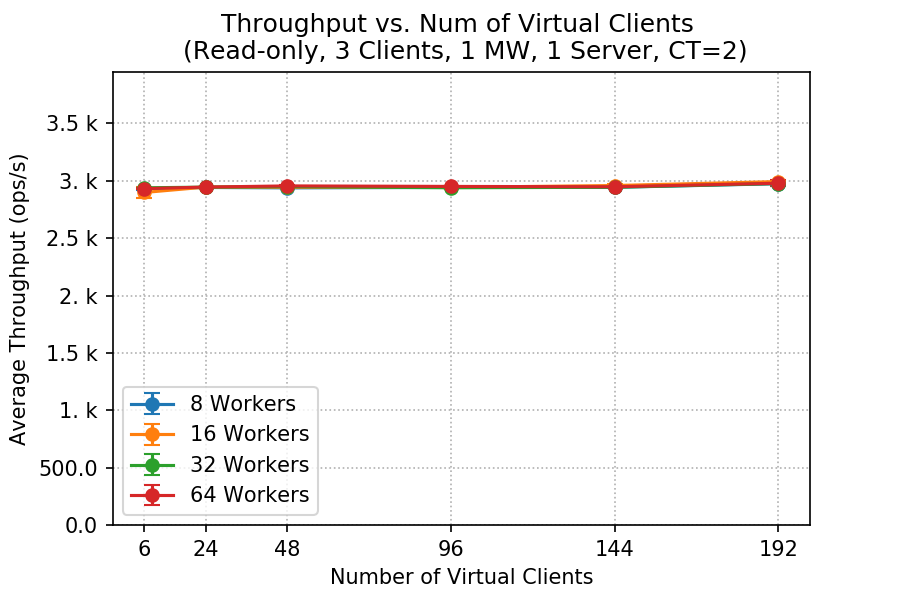
\includegraphics[width=1\linewidth]{figures/2_BaselineWithMW/one_mw/one_mw_tp_read_2018-12-06_23h08.png}
     \caption{Throughput of middleware}\label{one_mw_tp_read}
   \end{minipage}\hfill
   \begin{minipage}{0.48\textwidth}
     \centering
     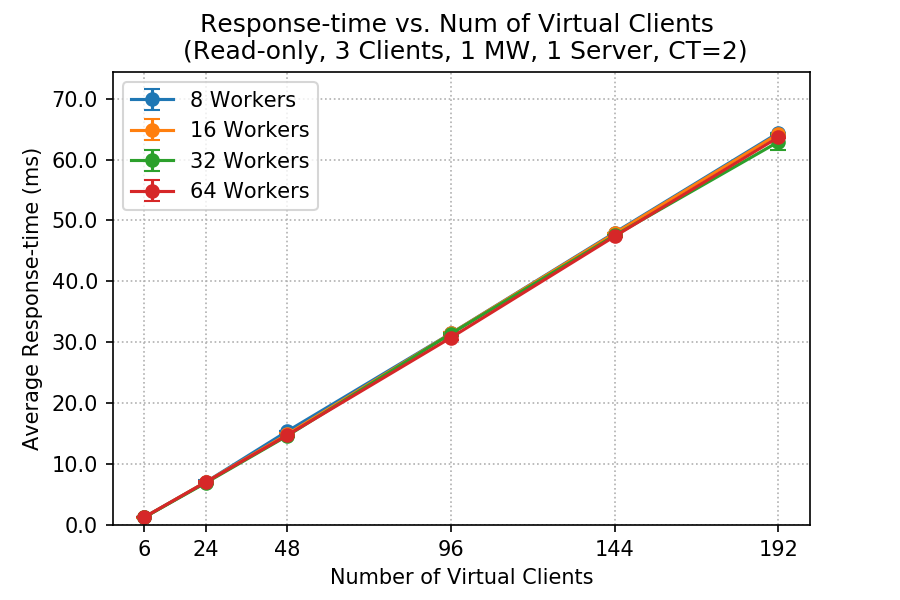
\includegraphics[width=1\linewidth]{figures/2_BaselineWithMW/one_mw/one_mw_rt_read_2018-12-06_23h08.png}
     \caption{Response time of middleware}\label{one_mw_rt_read}
   \end{minipage}
\end{figure}

%% explanation
% interactive law
The response time of the middleware is computed as the average time a request needs from the first encounter with the net-thread to the point where a worker thread sends the response back to the client. For the interactive law to hold, we can consider twice the network latency between the client and the middleware as the think time $Z$. 

% saturation & bottleneck
In Figure \ref{one_mw_tp_read} we can see that the saturation point for all worker settings is already reached at $6$ clients. The bottleneck of this setup is the outbound network bandwidth at the server, which can be seen in in Figure \ref{outbound_server_net_activity_one_mws}. Using \textit{iperf}, we checked that the maximum outbound network bandwidth of a server VM is 12.6 MBps, which is reached at $6$ clients and thus we don't see any under-saturation. The bottleneck also makes sense because of the large values the server has to send back for read-only workloads. Different number of workers reach the same maximum throughput, which supports the claim that bandwidth is the bottleneck because it is independent of the number of workers. 
\begin{figure}[H]
    \centering
	\includegraphics[scale=0.48]{figures/2_BaselineWithMW/one_mw/dstat_server_netsend_ratio_0:1_2018-12-06_23h08.png}
	\caption{Outbound network activity of the server VM.}
	\label{outbound_server_net_activity_one_mws}
\end{figure}
In the following, we want to support the claim by looking at the response time in more detail. Figure \ref{rt_breakdown_read_one_mw} shows that the response time stays the same for different number of workers, but the queue time shifts to the memcached RTT as we increase the number of workers. This is because we have a lower service rate of workers for small number of workers and thus requests wait longer in the middleware queue. If there are a lot of workers, requests are quickly dequeued, but they then congest at the server outbound queue and have to wait there instead because it is the bottleneck of the setup. 

\begin{figure}[H]
    \centering
	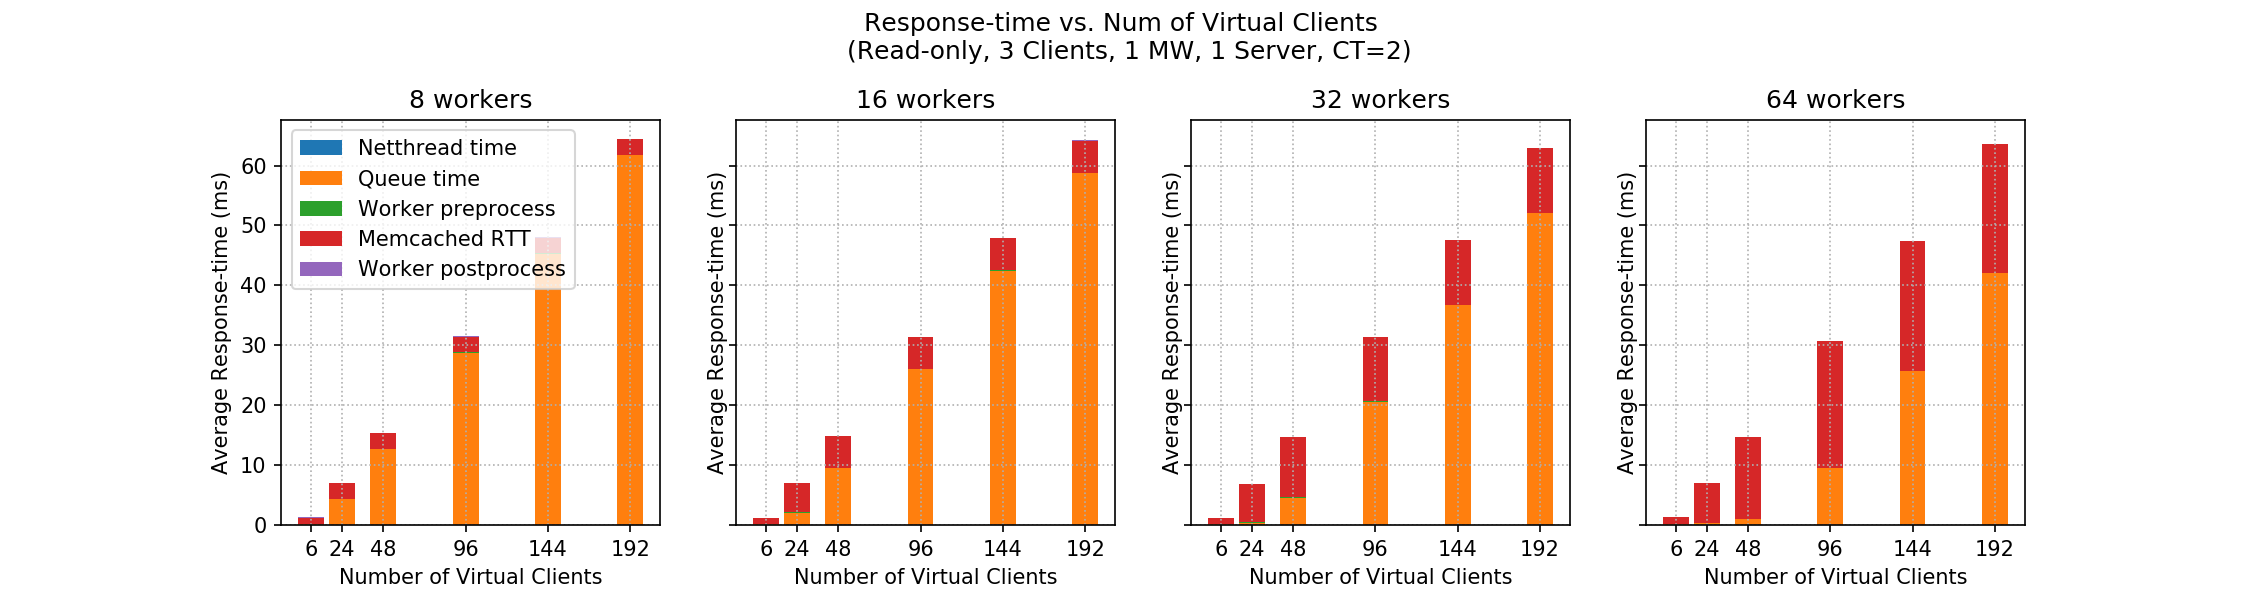
\includegraphics[scale=0.48,width=\linewidth]{figures/2_BaselineWithMW/one_mw/one_mw_rt_breakdown_read_2018-12-06_23h08.png}
	\caption{Response time breakdown of the read-only workloads.}
	\label{rt_breakdown_read_one_mw}
\end{figure}

$\bullet$ \textbf{Write-only load:} 
% plots
The throughput and response time measured on the middleware as a function of virtual clients for write-only workloads is shown in Figure \ref{one_mw_tp_write} and in Figure \ref{one_mw_rt_write}. 
\begin{figure}[ht]
   \begin{minipage}{0.48\textwidth}
     \centering
     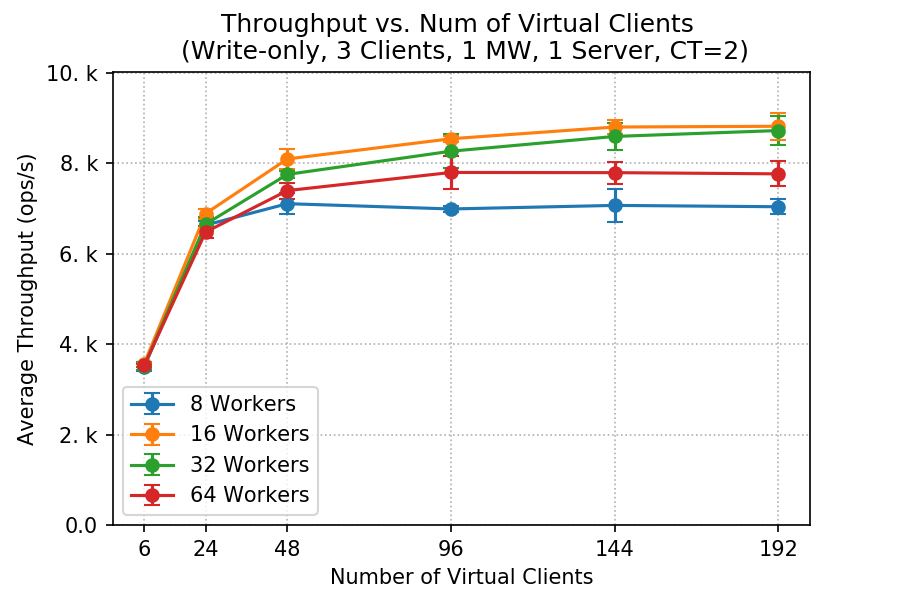
\includegraphics[width=1\linewidth]{figures/2_BaselineWithMW/one_mw/one_mw_mem_tp_write_2018-12-06_23h08.png}
     \caption{Throughput of middleware}\label{one_mw_tp_write}
   \end{minipage}\hfill
   \begin{minipage}{0.48\textwidth}
     \centering
     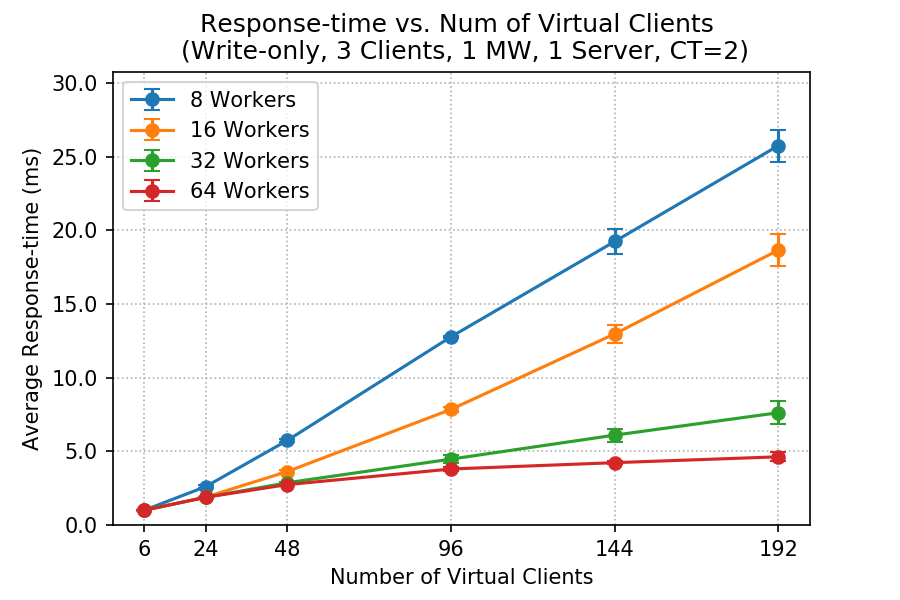
\includegraphics[width=1\linewidth]{figures/2_BaselineWithMW/one_mw/one_mw_rt_write_2018-12-06_23h08.png}
     \caption{Response time of middleware}\label{one_mw_rt_write}
   \end{minipage}
\end{figure}

%% explanation
% 8 and 16 worker threads
For \textbf{8 worker threads} saturation is reached at $24$ clients while for \textbf{16 worker threads} saturation is reached at $48$ clients as can be seen in Figure \ref{one_mw_tp_write} and \ref{one_mw_rt_write}. In both cases the bottleneck are the worker threads which cannot dequeue requests faster than they are enqueued by the net-thread. This can be verified by multiple metrics. First we can look at the average queue length for different number of clients. Figure \ref{queue_length_one_mw_write} shows that for 8 and 16 worker threads the queue length starts increasing more significantly at their saturation points. This happens because the arrival rate of requests into the queue is bigger than the overall service rate of the workers and thus requests start accumulating in the queue.   
\begin{figure}[H]
    \centering
	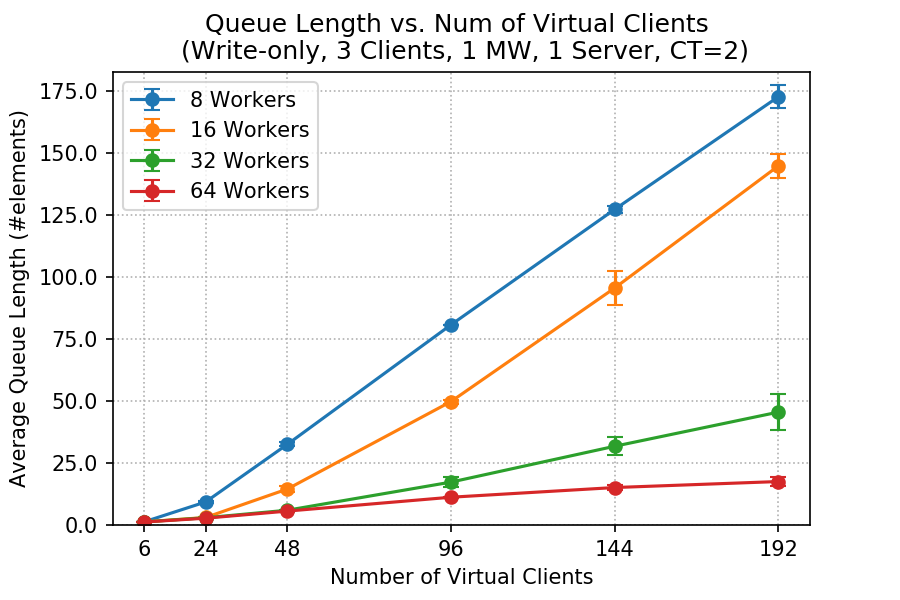
\includegraphics[scale=0.48]{figures/2_BaselineWithMW/one_mw/one_mw_queuelength_write_2018-12-06_23h08.png}
	\caption{Average queue length for write-only workloads.}
	\label{queue_length_one_mw_write}
\end{figure}
We can also look at the response time in the middleware in more detail. Figure \ref{rt_breakdown_write_one_mw} shows that for 8 and 16 worker threads, requests spend most of their time in the queue, and once dequeued they are processed quickly, which supports our claim. 
\begin{figure}[H]
    \centering
	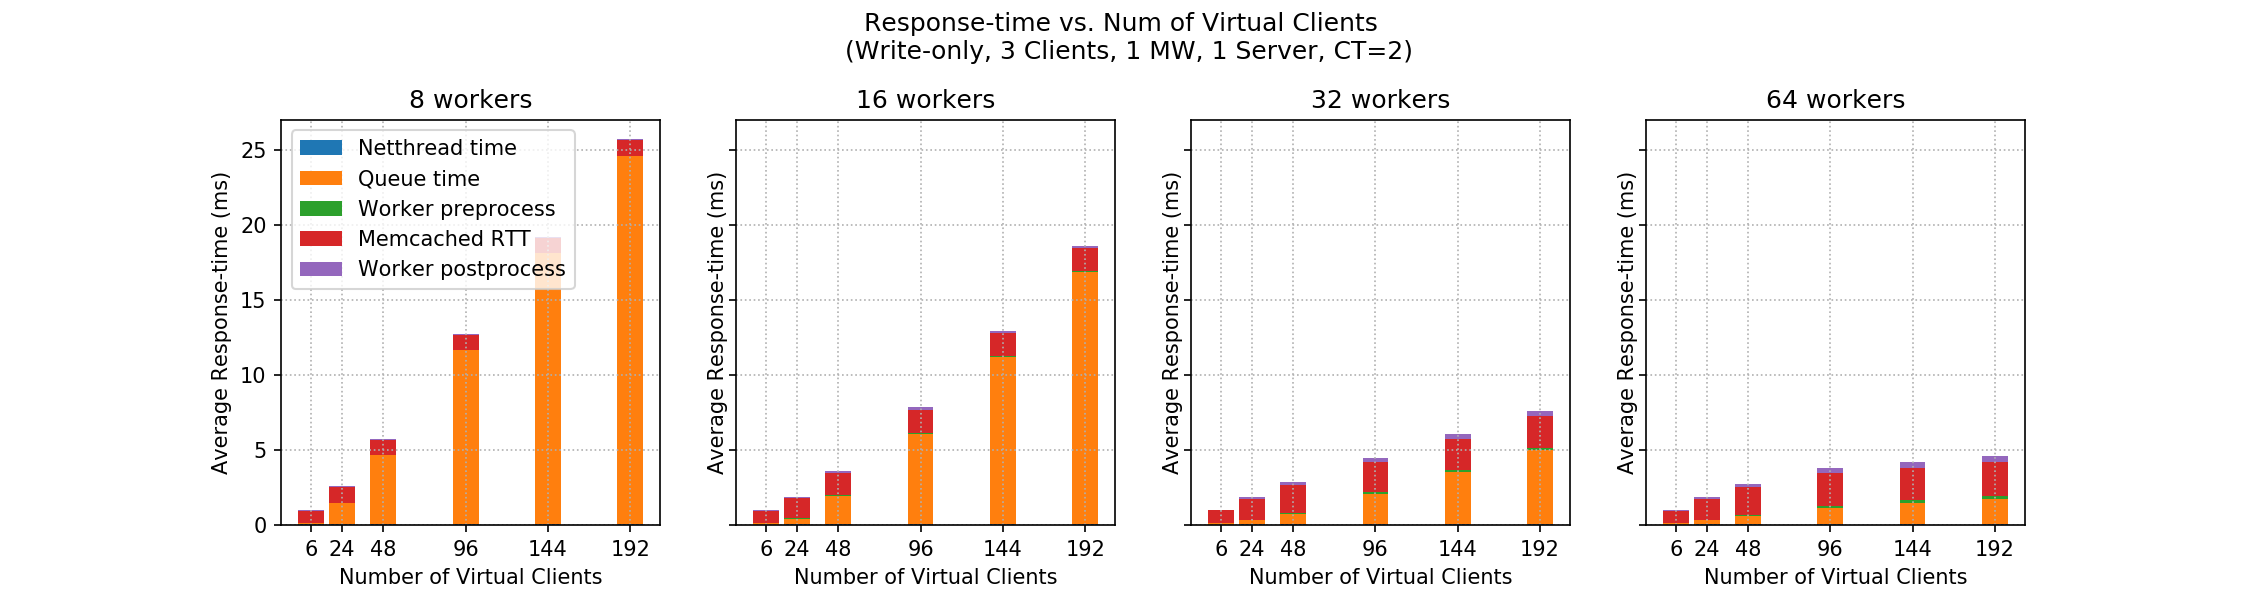
\includegraphics[scale=0.48,width=\linewidth]{figures/2_BaselineWithMW/one_mw/one_mw_rt_breakdown_write_2018-12-06_23h08.png}
	\caption{Response time breakdown of the write-only workloads.}
	\label{rt_breakdown_write_one_mw}
\end{figure}
% 32 and 64 worker threads
If we look at \textbf{32 and 64 worker threads}, first of all in Figure \ref{one_mw_tp_write} we see that in both cases saturation is reached at around 48 clients. The response time in the middleware for 32 and 64 worker threads is decreased in contrast to 8 and 16 worker threads as can be seen in Figure \ref{one_mw_rt_write}. This is because we increased the resources at the bottleneck, which are the worker threads. The queue time is decreased because the overall service rate of the workers is increased (Figure \ref{rt_breakdown_write_one_mw}).
Even though the response time at the middleware is decreased significantly, the overall response time measured at the clients (Figure \ref{rt_mem_write_one_mw}) did not, i.e. there is a new bottleneck now, which is the net-thread. Requests congest in the inbound network queue of the net-thread. 
This waiting time makes up roughly the difference between the response time measured on the middleware and on the client and is plotted separately in Figure \ref{netthread_queue_write}. We see that for 32 and 64 workers the time in front of the net-thread increases significantly at their saturation points.
\begin{figure}[H]
    \begin{minipage}{0.48\textwidth}
        \centering
	    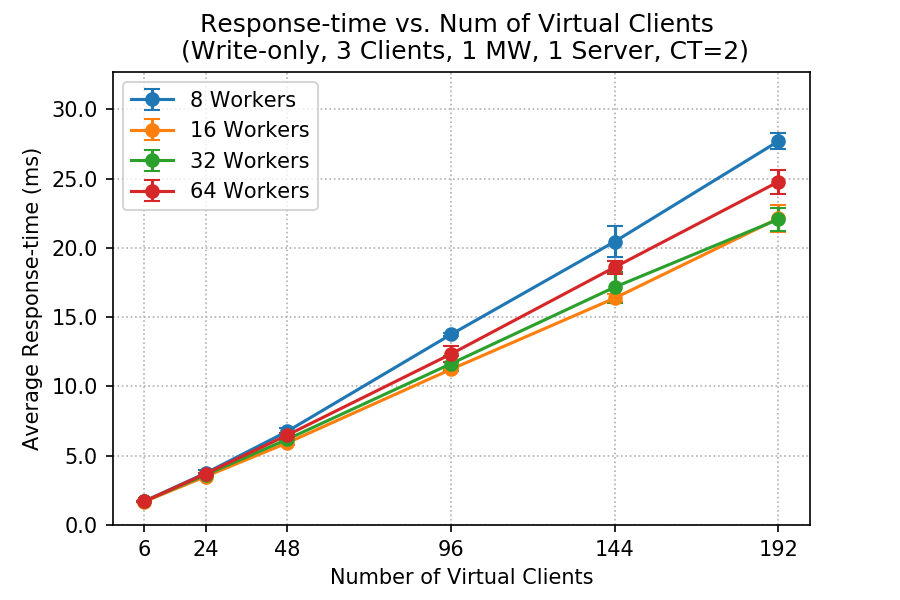
\includegraphics[scale=0.48]{figures/2_BaselineWithMW/one_mw/one_mw_mem_rt_write_2018-12-06_23h08.png}
	    \caption{Response time of the write-only workloads measured on client.}
	    \label{rt_mem_write_one_mw}
   \end{minipage}\hfill
   \begin{minipage}{0.48\textwidth}
        \centering
	    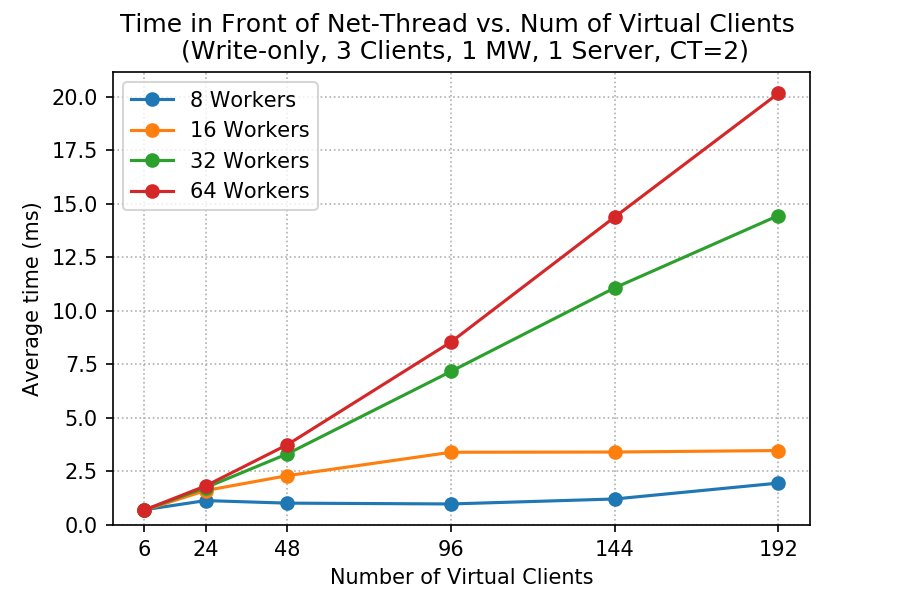
\includegraphics[scale=0.48]{figures/2_BaselineWithMW/one_mw/one_mw_rt_write_front_netthread_2018-12-06_23h08.png}
	    \caption{Average time spend in inbound network queue of net-thread.}
	    \label{netthread_queue_write}
   \end{minipage}
\end{figure}
The increase in inbound net-thread queue time for higher number of workers can be explained as follows: The more worker threads we have, the higher the overhead on the CPU i.e. more threads compete for the same resource and thus there are more context switches (verified with \textit{dstat}), which affects the performance of the net-thread because it gets less CPU time and can process fewer requests. Note that workers are allocated a priori in our system.

So even tough going from 16 to 32 worker threads removes the worker bottleneck and decreases queue time (Figure \ref{rt_breakdown_write_one_mw}), this time is compensated by the increased waiting time in front of the net-thread, and thus the throughput does not improve (Figure \ref{one_mw_tp_write}). Going from 32 to 64 worker threads has almost no effect on the response time at the middleware because already 32 worker threads were enough to handle the load. So we just have more net-thread waiting time because of the higher overhead on the CPU but without decreased queue time. This leads to a worse throughput than in the 32 worker thread case (Figure \ref{one_mw_tp_write}).


\subsection{Two Middlewares} \label{sec:baselineWithMWTwo}
% setup description
In this experiment we connect one load generator machine (two instances of memtier with CT=1) to two middlewares and use 1 memcached server. 
The overview of the experiment parameters is given in the following table:
\begin{center}
	\scriptsize{
		\begin{tabular}{|l|c|}
			\hline Number of servers                & 1                        \\ 
			\hline Number of client machines        & 3                        \\ 
			\hline Instances of memtier per machine & 2                        \\ 
			\hline Threads per memtier instance     & 1                        \\
			\hline Virtual clients per thread       & \{1,4,8,16,24,32,40\}       \\ 
			\hline Workload                         & Write-only and Read-only \\
			\hline Number of middlewares            & 2                        \\
			\hline Worker threads per middleware    & \{8,16,32,48\}              \\
			\hline Repetitions                      & 3                        \\ 
			\hline 
		\end{tabular}
	} 
\end{center}

$\bullet$ \textbf{Read-only load:} 
% plots
The throughput and response time as a function of virtual clients for read-only workloads is shown in Figure \ref{two_mws_tp_read} and in Figure \ref{two_mws_rt_read}. 
\begin{figure}[H]
   \begin{minipage}{0.48\textwidth}
     \centering
     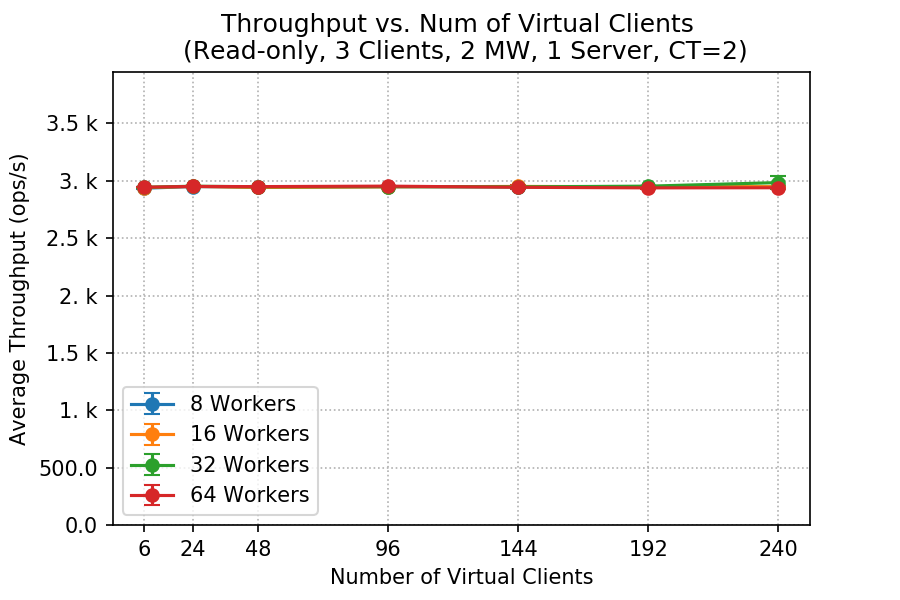
\includegraphics[width=1\linewidth]{figures/2_BaselineWithMW/two_mws/two_mws_tp_read_2018-12-07_09h02.png}
     \caption{Throughput of middlewares}\label{two_mws_tp_read}
   \end{minipage}\hfill
   \begin{minipage}{0.48\textwidth}
     \centering
     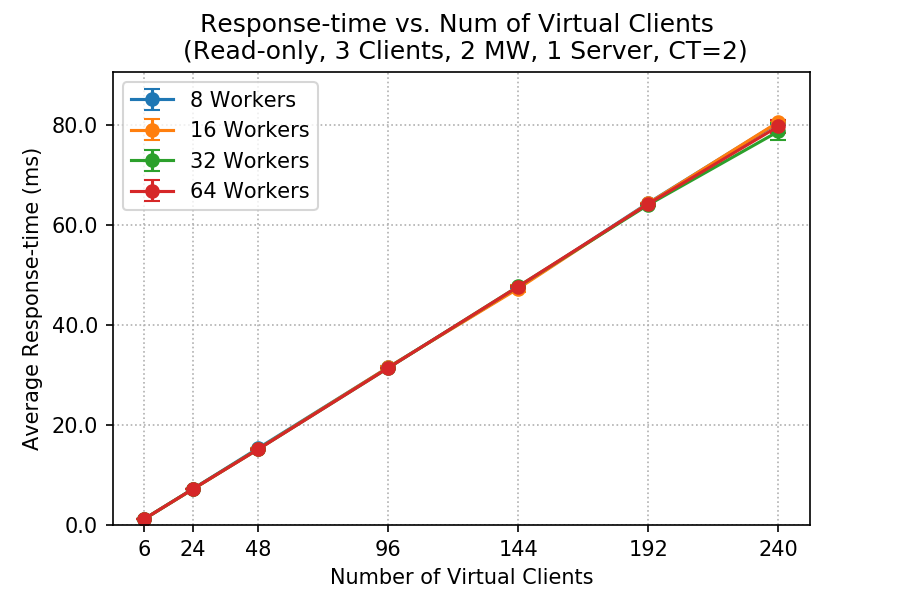
\includegraphics[width=1\linewidth]{figures/2_BaselineWithMW/two_mws/two_mws_rt_read_2018-12-07_09h02.png}
     \caption{Response time of middlewares}\label{two_mws_rt_read}
   \end{minipage}
\end{figure}

%% explanation
In Figure \ref{two_mws_tp_read} we can see that the saturation point for all worker settings is already reached at $6$ clients. The bottleneck of this setup is the same as for the one middleware case, namely the outbound network bandwidth at the server, which can be seen in in Figure \ref{outbound_server_net_activity_two_mws}. This also makes sense because going from one middleware to two middlewares does not improve the bottleneck at the server. The same reasoning done for the bottleneck analysis in the one middleware case applies here. 
\begin{figure}[H]
    \centering
	\includegraphics[scale=0.48]{figures/2_BaselineWithMW/two_mws/dstat_server_netsend_ratio_0:1_2018-12-07_09h02.png}
	\caption{Outbound network activity of the server VM.}
	\label{outbound_server_net_activity_two_mws}
\end{figure}
We can also look at the response time in more detail (Figure \ref{rt_breakdown_read_two_mws}) and see that increasing the number of workers shifts the time spent in the queue to the time spent in the outbound network queue of the server because of the server bandwidth bottleneck. 
\begin{figure}[H]
    \centering
	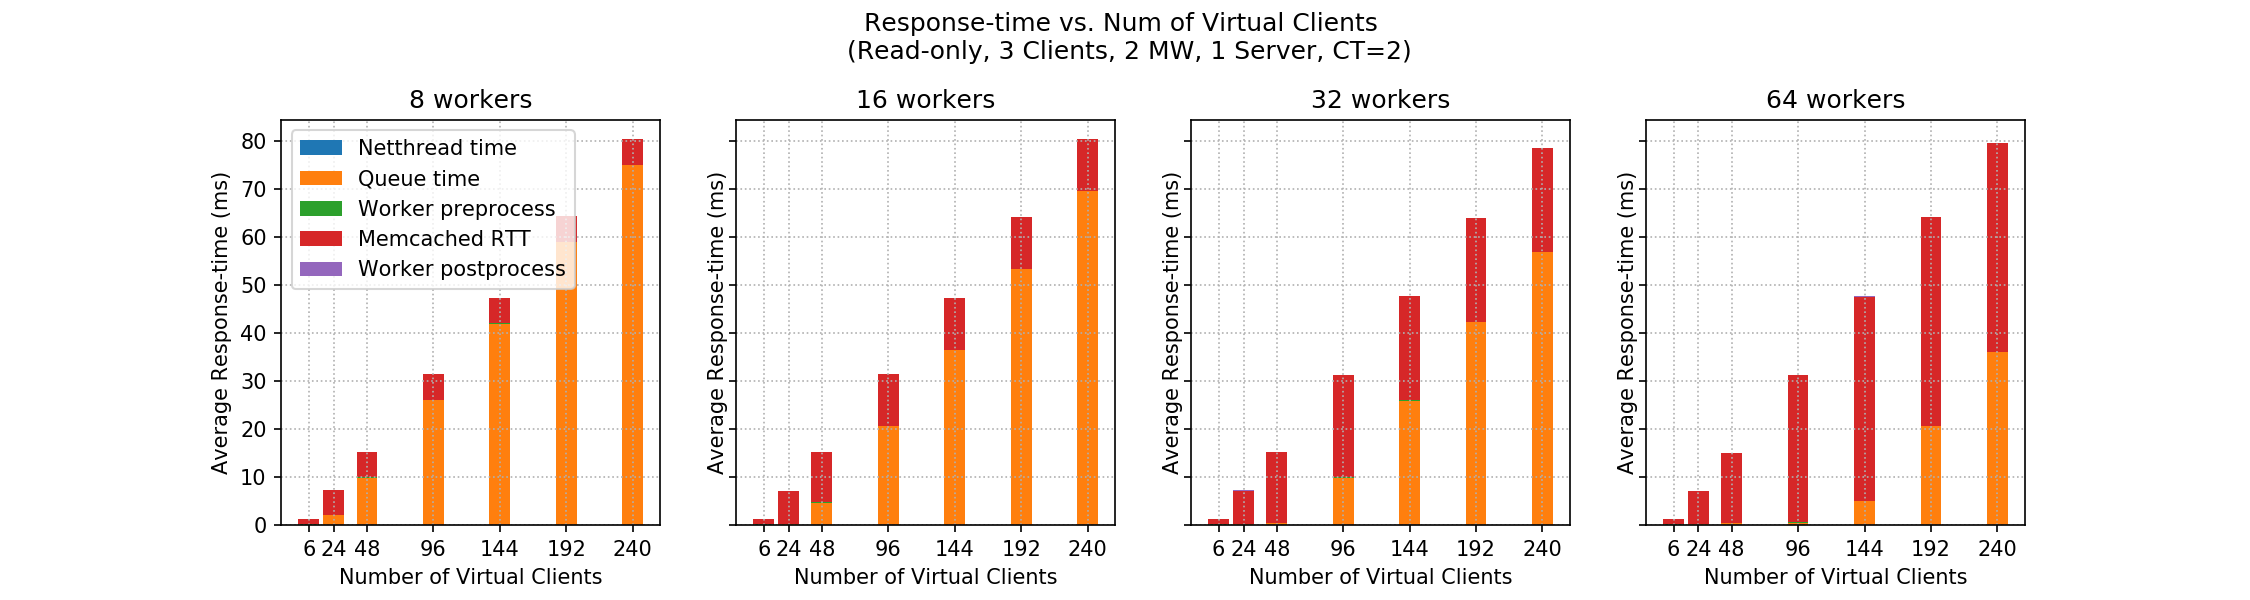
\includegraphics[scale=0.48,width=\linewidth]{figures/2_BaselineWithMW/two_mws/two_mws_rt_breakdown_read_2018-12-07_09h02.png}
	\caption{Response time breakdown of the read-only workloads.}
	\label{rt_breakdown_read_two_mws}
\end{figure}

$\bullet$ \textbf{Write-only load:} 
% plots
The throughput and response time as a function of virtual clients for write-only workloads is shown in Figure \ref{two_mws_tp_write} and in Figure \ref{two_mws_rt_write}. 
\begin{figure}[H]
   \begin{minipage}{0.48\textwidth}
     \centering
     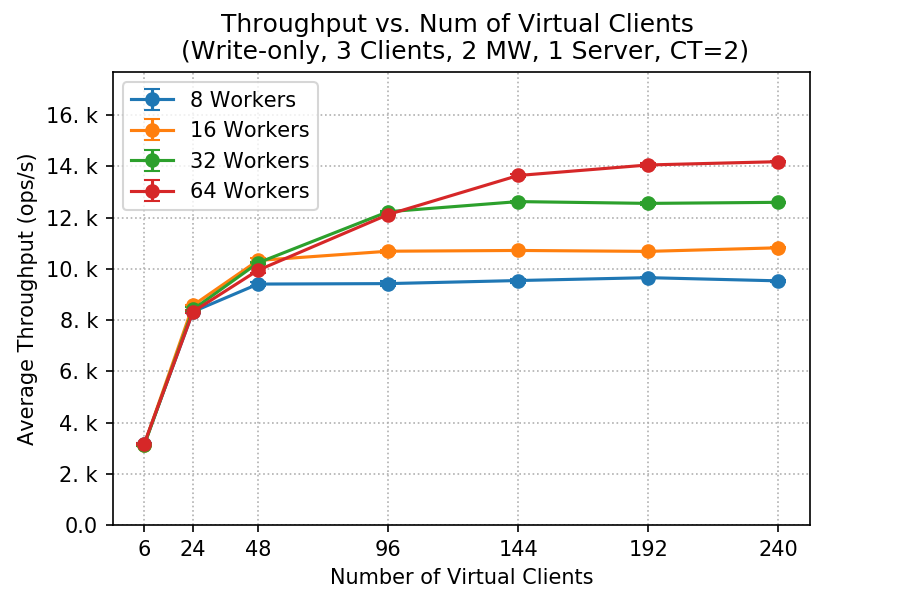
\includegraphics[width=1\linewidth]{figures/2_BaselineWithMW/two_mws/two_mws_tp_write_2018-12-07_09h02.png}
     \caption{Throughput of middlewares}\label{two_mws_tp_write}
   \end{minipage}\hfill
   \begin{minipage}{0.48\textwidth}
     \centering
     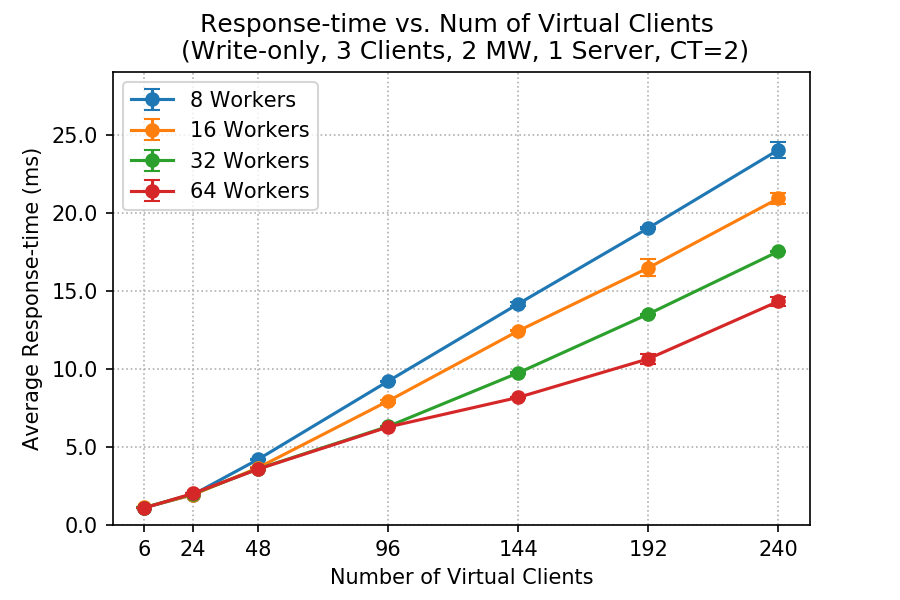
\includegraphics[width=1\linewidth]{figures/2_BaselineWithMW/two_mws/two_mws_rt_write_2018-12-07_09h02.png}
     \caption{Response time of middlewares}\label{two_mws_rt_write}
   \end{minipage}
\end{figure}
%% explanation
Looking at Figure \ref{two_mws_tp_write}, we see that saturation for 8 workers is reached at $24$ clients, for 16 workers at $48$ clients, for 32 clients at $96$ clients and for 64 workers at $144$ clients because at those points throughput starts to flatten. The saturation points are confirmed later in the analysis. In the one middleware case the net-thread is the bottleneck, but having two middlewares removes the net-thread bottleneck because we now have two net-threads sharing the same load. This can be confirmed by looking at the response time graph computed from the memtier outputs, which looks exactly the same as Figure \ref{two_mws_rt_write} plus 1-2 ms for the network latency between the client and the middleware. Thus no time is lost in front of the net-thread anymore. 
The bottleneck of this setup are the worker threads. To see this we can first look at the average queue length (Figure \ref{queue_length_two_mws_write}). The queue length starts increasing significantly at the mentioned saturation points.
We also checked the CPU utilization of the server VM (seen in Figure \ref{cpu_two_mws_write}) to verify that it does not reach full utilization which means that it is not the bottleneck of this setup.

%For 8, 16 and 32 workers the queue length starts increasing significantly at the mentioned saturation points. Actually for 64 worker threads the workers are not the bottleneck anymore but we claim that the single memcached thread is at its limit because it has to serve a lot of workers simultaneously.
%The server reaches almost full utilization at 144 clients as can be seen in Figure \ref{cpu_two_mws_write}.

\begin{figure}[H]
    \begin{minipage}{0.48\textwidth}
        \centering
	    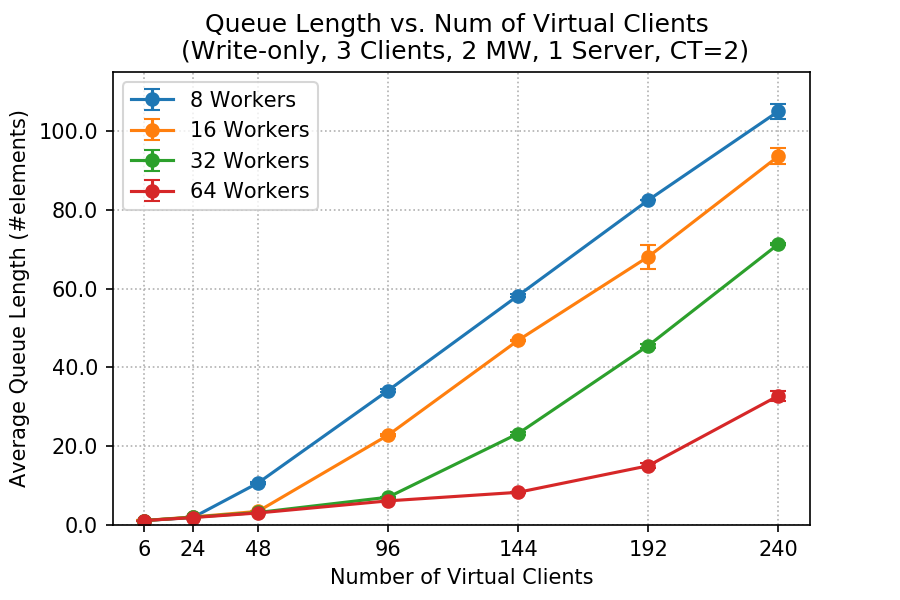
\includegraphics[scale=0.48]{figures/2_BaselineWithMW/two_mws/two_mws_queuelength_write_2018-12-07_09h02.png}
	    \caption{Average queue length for write-only workloads.}
	    \label{queue_length_two_mws_write}
    \end{minipage}\hfill
    \begin{minipage}{0.48\textwidth}
        \centering
	    \includegraphics[scale=0.48]{figures/2_BaselineWithMW/two_mws/dstat_server_cpu_ratio_1:0_2018-12-07_09h02.png}
	    \caption{CPU utilization of server VM for write-only workloads.}
	    \label{cpu_two_mws_write}
    \end{minipage}
\end{figure}

We can support our claim by additionally looking at the response time of the middleware in more detail (Figure \ref{rt_breakdown_write_two_mws}). We can see that the queue time starts increasing at the saturation points because the arrival rate of requests into the queue is higher then the service rate of the workers together. Note that if we fix the workers and look at the memcached RTT during saturation while increasing the clients, we see that it stays constant. That is because the workers are at full utilization and the arrival rate of requests into the memcached queue does not increase anymore, which further supports our claim that the workers are the bottleneck. 

%We can see that in deed for 8,16 and 32 workers the queue time makes up most of the response time. 64 workers have a higher service rate than arrival rate of requests into the queue and thus the queue time almost disappears. The bottleneck at the server leads to an increased memcached RTT for the 64 workers case which supports our claim. 
\begin{figure}[H]
    \centering
	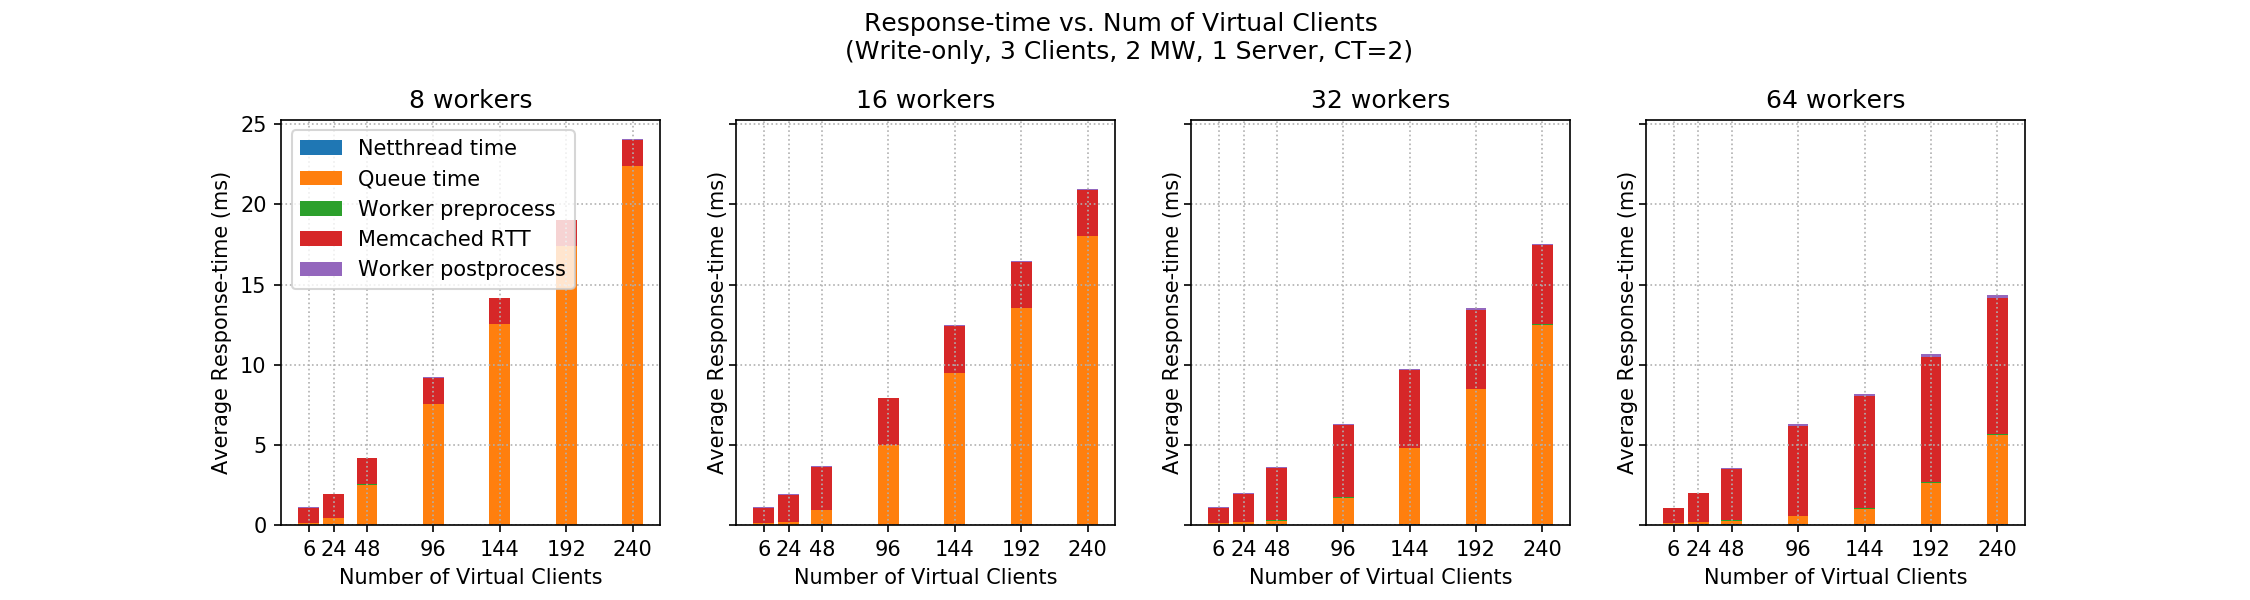
\includegraphics[scale=0.48,width=\linewidth]{figures/2_BaselineWithMW/two_mws/two_mws_rt_breakdown_write_2018-12-07_09h02.png}
	\caption{Response time breakdown of the write-only workloads.}
	\label{rt_breakdown_write_two_mws}
\end{figure}
\subsection{Summary}
\begin{center}
	{Maximum throughput for one middleware.}
	\begin{tabular}{|p{5.7cm}|p{2.1cm}|p{1.9cm}|p{1.9cm}|p{1.9cm}|}
		\hline                                & Throughput & Response time  & Average queue time & Miss rate  \\ 
		\hline Reads: Measured on middleware  &2'929 ops/s &1.26ms&      0.1ms &  0.0\%        \\ 
		\hline Reads: Measured on clients     & 2'925 ops/s&   2.06ms    & n/a   &   0.0\%    \\ 
		\hline Writes: Measured on middleware &   8'105 ops/s & 3.63ms         &    1.87ms      & n/a   \\ 
		\hline Writes: Measured on clients    &  8'097 ops/s&  5.93ms           & n/a                   & n/a      \\ 
		\hline 
	\end{tabular}
\end{center}

\begin{center}
	{Maximum throughput for two middlewares.}
	\begin{tabular}{|p{5.7cm}|p{2.1cm}|p{1.9cm}|p{1.9cm}|p{1.9cm}|}
		\hline                                & Throughput & Response time & Average queue time & Miss rate \\ 
		\hline Reads: Measured on middleware  &   2'935 ops/s &  1.18ms     &    0.08ms      & 0.0 \%   \\ 
		\hline Reads: Measured on clients     &   2'923 ops/s  &  2.06ms       & n/a         &   0.0 \%  \\ 
		\hline Writes: Measured on middleware &   13'645 ops/s &  8.18ms      &      0.97 ms              & n/a       \\ 
		\hline Writes: Measured on clients    &   13'603 ops/s   &10.6ms        & n/a                   & n/a     \\ 
		\hline 
	\end{tabular}
\end{center}
% table: 6 clients and 8 workers for read in both. 48 clients,16 workers for write one mw. 14 clients, 64 workers for write in two mw.
% conclusions
First note that again the maximum throughput is chosen by also taking the latency into consideration.
For the read-only workload, we choose the lowest number of clients (and workers) in both cases because the throughput remains the same while the response time increases with more clients. For the write-only workload and one middleware configuration, we choose $48$ clients and $16$ workers because going even further to $96$ clients would only increase the throughput by $5.5\%$ while increasing the response time more significantly by $89.5\%$. For the write-only workload and two middlewares configuration, we choose $144$ clients and $64$ workers because going to $192$ clients would only increase the throughput by $3\%$ but at the same time increase response time by $34.4\%$.

The response time difference between the client and the middleware is due to the time a request spends between a client and the middleware, which is not part of the response time measured at the middleware. 

If we look at the read-workloads, we see that increasing the number of middlewares does not improve the throughput. This is because the bottleneck is the outbound network bandwidth at the server, which puts a hard limit on the achievable throughput. 

If we look at the write-workloads, we see that going from one to two middlewares significantly increases the throughput. This is because the bottleneck in the one middleware case is the net-thread and having two net-threads allows them to share the same load, which reduces their utilization. 




